\chapter{PACORA Framework}
%------------------------------------------------------------------------------------------------------------------------------------------------------------------------
\section{Introduction}
%------------------------------------------------------------------------------------------------------------------------------------------------------------------------
\pacora is a framework designed to determine the proper amount of each
resource type to give each application.  The purpose of \pacora is to dynamically assign resources
across multiple applications to guarantee responsiveness without
over-provisioning and to adapt allocations as the application mix
changes. For example, consider a video conference scenario where each participant requires a separate,
performance-guaranteed video stream.  New participants may join the
conference and others may leave, increasing or decreasing the number
of streams running at any given time.  Simultaneously, participants
may be collaborating through web browsers, or watching shared video
clips and web searching, while their systems run compute-intensive
background tasks such as updates, virus scans, or file indexing.
Although it may be relatively straightforward to provide
responsiveness guarantees for individual applications such as video
streams, the real challenge is to do so without reserving excessive
resources, which will compromise system utilization, power
consumption, or responsiveness of other applications.

We believe \pacora is applicable to many resource-allocation
scenarios, from cloud providers determining how many resources to give
each job to avoid violating Service-Level Agreements (SLAs), through databases allocating
resources to queries, to distributed embedded systems allocating
bandwidth among devices and sensors.  These potential applications of \pacora are discussed in greater detail in Chapter~\ref{discuss}. In this chapter, we describe the mathematical formulation of the \pacora framework, prove the convexity, and present our initial evaluations of the potential of using \pacora for resource allocation in an operating system.

%------------------------------------------------------------------------------------------------------------------------------------------------------------------------
\section{\pacora Architecture}\label{sys_design}
%------------------------------------------------------------------------------------------------------------------------------------------------------------------------
\pacora formulates resource allocation as an optimization problem
built from two types of application-specific functions: a
response-time function and a penalty function. The response-time
function represents the performance of the application with different
resources and is built with runtime measurements.  The penalty
function represents the user-level goals for the application
(\emph{i.e.,} the deadline and how important it is to meet). \pacora uses convex optimization~\cite{BoVa} to
determine the ideal resource allocation across all active
applications.  The following subsections briefly introduce the primary
components of \pacora and the optimization formulation.

\subsection{Response-Time Functions}

Response-time functions (RTF) represent the expected \emph{response
  time} of an application as a function of the resources allocated to
the application. The response time is an application-specific measure
of the performance of the application.  For example, the response time
of an application might be:
    \begin{itemize}\itemsep0pt \parskip0pt \parsep5pt
    \item The time from a mouse click to its result;
    \item The time to produce a frame;
    \item The time from a service request to its response;
    \item The time from job launch to job completion;
    \item The time to execute a specified amount of work.
    \end{itemize}

The RTFs are built to be convex functions.  All applications have a
function of the same form, but the application-specific weights are set
using the performance history of the application.  RTFs are designed
to capture information such as how well an application scales with a
particular resource. As a result, RTFs naturally support
heterogeneity.  Each CPU or GPU type is simply viewed as a different
resource type by the system, and thus the RTFs will represent how
effectively an application uses a particular type of
core. Figure~\ref{sample_rtf} shows two example RTFs we have created
from applications we studied.

\begin{figure*}[hb]
\subfloat{
\includegraphics*[bb=0 0 360 360,width=.48\columnwidth]{Figures/bfs-fig.pdf}
\label{bfs-fig}
}
\subfloat{
\includegraphics*[bb=0 0 360
  360,width=.48\columnwidth]{Figures/streamcluster-fig.pdf}
\label{streamcluster-fig}
}  
\caption{\label{sample_rtf} Response-Time Functions for a
  breadth-first search algorithm and \texttt{streamcluster} from the PARSEC benchmark suite~\cite{parsec}. We show two resource dimensions: cores and cache ways.}
\end{figure*}

Equation~\ref{rtf_eq} below shows the RTF we selected for \pacora.  

\begin{equation}\label{rtf_eq}
\tau(w,a) = \tau_0 + \sum_{i\in n,j\in n}{\frac{w_{i,j}}{\sqrt{a_i * a_j}}}
\end{equation}

Here $\tau$ is the response time, $i$ and $j$ are
resource types, $n$ is the total number of resource types,
$a_{i}$ and $a_{j}$ are the allocations of resource types $i$
and $j$, and $w_{i,j}$ is the application-specific weight for
the term representing resources $i$ and $j$.

In our experience the cross term weights (those with $i\neq j$) are almost always negligible and can be omitted if desired.
This omission allows the dimensionality of the function, and thus the storage space required, to increase roughly linearly with the number of resource types.  The value of the cross terms is discussed further in Section~\ref{init_eval}.

We chose this specific function because it is convex in the resources, and in initial application studies,
we found it models response time behavior accurately enough to allow the optimization to make good decisions. Section~\ref{RTFs} describes the design considerations for the RTFs in more detail. Section~\ref{init_eval} shows these evaluation results and discusses alternative models that were considered and evaluated during the design process.

\subsection{Penalty Functions}

Penalty functions are designed to represent the user-level goals of
the application. They are similar to priorities but are functions of
the response time rather than simply values, so they can explicitly
represent deadlines.  Knowing the deadlines lets the system make
optimizations that are difficult in today's systems, such as running
just fast enough to make the deadline. Like priorities, the penalty
functions are set by the system on behalf of the user.


\begin{figure}[hb]
\parbox{3in}{
\includegraphics*[width=.45\columnwidth]{Figures/Penalty1.eps}
\caption{\label{f:pen1}A penalty function with a response time constraint.}
}
\hspace{\fill}
\parbox{3in}{
\includegraphics*[width=.45\columnwidth]{Figures/Penalty2.eps}
\caption{\label{f:pen2}A penalty function with no response time constraint.}
}
\end{figure}

\pacora's penalty functions $\pi$ are non-decreasing piecewise-linear
functions of the response time $\tau$ of the form $\pi(\tau) = \max(0, (\tau - d)s)$
where $d$ represents the deadline of the application and $s$ (slope)
defines the rate the penalty increases as response time increases. For
applications without response-time constraints the deadline can be set
to $0$. Two representative graphs of this type appear in
Figures~\ref{f:pen1} and~\ref{f:pen2}.

\subsection{Resource Allocation as Optimization}

\pacora formulates resource allocation as an optimization problem
designed to minimize the total penalty of the system. This approach is
analogous to minimizing user dissatisfaction with the user experience
due to missed deadlines in a client system and minimizing the contract
penalties paid for violated SLAs in a cloud
system.

The optimization selects the allocations for all resources and
resource types at once.  This approach enables the system to make
tradeoffs between resource types.  For example, the system could
choose to allocate more memory bandwidth in lieu of on-chip cache, or
one large core instead of several small cores.  Given that all of the
resources allocated to an application contribute to the response time,
it would difficult to provide predictable response times for
applications without over-provisioning by independently allocating each resource type.

A succinct mathematical characterization of this resource allocation scheme is the following:
\begin{eqnarray}
& \makebox[1in][r]{Minimize}   & \sum_{p\in P} {\pi_p(\tau_p(a_{p,1}\ldots a_{p,n}))}  \\
& \makebox[1in][r]{Subject to} & \sum_{p\in P} a_{p,r} \leq A_r, r = 1,\ldots n        \\
& \makebox[1in][r]{and}        & a_{p,r} \geq 0
\end{eqnarray}
Here $\pi_p$ is the penalty function for application $p$,
$\tau_p$ is its response time function,
$a_{p,r}$ is the allocation of resource $r$ to application $p$,
and $A_r$ is the total amount of resource $r$ available. 

\subsection{Managing Power and Energy}
In \pacora, we create an artificial application to represent the
interest in reducing the power and energy of the system.  Application 0 is
designated the idle application and receives allocations of all
resources that are left idle, \emph{i.e.,} not allocated to other
applications.  If the system has the appropriate power management mechanisms, these idle resources can be powered off or put to sleep to save power.

Additionally, application 0 functions as \emph{slack} variables in our optimization problem turning the resource bounds into equalities:
\begin{equation}
\sum_{p\in P} a_{p,r} - A_r = 0, r = 1,\dots n.
\end{equation}

The ``response time'' for application 0, $\tau_0$, is artificially
defined to be the total system power consumption.  Application 0's RTF represents how the system power improves when particular resources are left idle (\emph{i.e.,} allocated to application 0), which is similar to other RTFs since they represent how the response time of an application improves when allocated particular resource types. This response function is affine and monotone non-increasing in its arguments $a_{0,r}$.

The penalty function $\pi_0$ establishes a system tradeoff between
power and performance that will determine which resources are
allocated to applications to improve performance and which are left
idle.  The penalty function $\pi_0$ can be used to keep total system
power below the parameter $d_0$ to the extent the penalties of other
applications cannot overcome its penalty slope $s_0$. Both $s_0$ and
$d_0$ can be adjusted to reflect the current battery charge in mobile
devices. For example, as the battery depletes, $d_0$ could be decreased or $s_0$ increased
to force other applications to slow or cease execution.


%------------------------------------------------------------------------------------------------------------------------------------------------------------------------
\section{Convex Optimization}
%------------------------------------------------------------------------------------------------------------------------------------------------------------------------
If the penalty functions, response time functions, and resource
constraints were arbitrary, little could be done to optimize the total
penalty beyond searching at random for the best allocation.  However, we designed \pacora to be convex by construction, which enables us to use convex optimization~\cite{BoVa} methods to solve the optimization. 
By framing our resource allocation problem as a convex optimization problem, we get two significant benefits: for each problem an optimal
solution exists without multiple local extrema, and fast optimization methods with practical incremental solutions become feasible.  In this section, we prove the convexity of \pacora's optimization formulation and the penalty and RTF functions. \pacora also formulates RTF \emph{creation} as a convex optimization
problem, as explained in Section~\ref{rtf_creation}.

\subsection{Resource Allocation Optimization Convexity}

A constrained optimization problem is \emph{convex} if both the objective function to be minimized
and the constraint functions that define its feasible solutions are convex functions.
A function $f$ is convex if its domain is a convex set and
$f(\theta x + (1-\theta)y) \leq \theta f(x) + (1-\theta)f(y)$
for all $\theta$ between 0 and 1.
A set is convex if for any two points $x$ and $y$ in the set, the point
$\theta x + (1-\theta)y$
is also in the set for all $\theta$ between 0 and 1.
If $f$ is differentiable, it is convex if its domain is an open convex set and
$f(y) \geq f(x) + \nabla f^T\cdot(y-x)$ where $\nabla f$ is the gradient of $f$.
Put another way, $f$ is convex if its first-order Taylor approximations
are always global underestimates of its true value.

A convex optimization problem is one that can be expressed in this form:
\begin{eqnarray*}
& \makebox[1in][r]{Minimize}   & f_0(x_1,\ldots x_m)                              \\
& \makebox[1in][r]{Subject to} & f_i(x_1,\ldots f_m) \leq 0, i = 1,\ldots k        \\
& \makebox[1in][r]{where}      & \forall i \quad f_i:\Re^m \rightarrow \Re \mbox{ is convex.}
\end{eqnarray*}


\pacora's resource allocation problem can be transformed into a convex
optimization problem in the $m = |P|\cdot n$ variables $a_{p,r}$ as
long as the penalty functions $\pi_p$ are convex non-decreasing and
the response-time functions $\tau_p$ are convex.  We designed our
functions to meet these constraints, and proofs of their convexity are shown below.
 
The resource constraints are affine and therefore convex; they can be rewritten as 
\begin{equation}
\sum_{p\in P} (a_{p,r} - A_r) \leq 0  -a_{p,r} \leq 0
\end{equation}
\begin{equation}
-a_{p,r} \leq 0
\end{equation}

The convex formulation makes the optimization scale linearly in the
number of resource types and the number of applications.  For client
operating systems with around 100 applications running and 10 resource
dimensions, the total number of variables in the optimization problem
is 1000---a very small problem which is solved in microseconds on
current systems.  Cloud systems could have many more than 100
applications running, but the problem size scales linearly and the
potential benefits of a good allocation should scale rapidly with the
size of the system.

\subsection{Penalty Function Convexity}
In this section, we discuss the convexity of \pacora's penalty functions.
A few facts about convex functions will be useful in what follows.
First, a \emph{concave} function is one whose negative is convex.
Maximization of a concave function is equivalent to minimization of its convex negative.
An affine function, one whose graph is a straight line in two dimensions or a hyperplane in n dimensions,
is both convex and concave.  A non-negative weighted sum or point-wise maximum (minimum) of convex (concave) functions is convex (concave), as is either kind of function composed with an affine function.  The composition of a convex non-decreasing (concave non-increasing) scalar function with a convex function remains convex (concave).

Each penalty function $\pi$ is the pointwise maximum of two affine functions and is therefore convex.
Moreover, since each penalty function is scalar and nondecreasing,
its composition with a convex response time function will also be convex.

\subsection{Response Time Convexity}
We now show that response time functions $\tau$ including the various bandwidth amplification functions are convex
in both the bandwidth and memory resources $b_r$ and $m_r$ given any of the possibilities we have considered.
Since norms preserve convexity, this reduces the question to proving each term in the norm is convex.
Since all quantities are positive and both maximum and scaling by a positive constant preserve convexity,
\begin{eqnarray*}
\lefteqn{w/(b\cdot\min(c_1\alpha_1(m),c_2\alpha_2(m)))}   \\
&=& \max(w/(b\cdot c_1\alpha_1(m)),w/(b\cdot c_2\alpha_2(m))).
\end{eqnarray*}
It therefore only remains to show that both $1/\sqrt{b\cdot m}$ and $1/(b\cdot\alpha(m))$ are convex in $b$ and $m$.

A function is defined to be \emph{log-convex} if its logarithm is convex.
A log-convex function is itself convex because exponentiation preserves convexity,
and the product of log-convex functions is convex because the log of the product is the sum of the logs,
each of which is convex by hypothesis.
Now $1/b$ is log-convex for $b > 0$ because $-\log b$ is convex on that domain.
In a similar way, $\log(1/\sqrt{b\cdot m}) = -(\log b + \log m)/2$
and $\log m^{-1/d} = -(\log m)/d$ are convex.
Finally, $\log (1/\log m)$ is convex because its second derivative is positive for $m > 1$:
\begin{eqnarray*}
\frac{d^2}{dm^2}\log (1/\log m) &=& \frac{d^2}{dm^2}(-\log\log m)  \\
                                  &=& \frac{d}{dm}\left(\frac{-1}{m\log m}\right) \\
                                  &=& \frac{1 + \log m}{(m\log m)^2}.
\end{eqnarray*}

Summing up, a response time function for a application might be modeled by the convex function
\begin{eqnarray*}
\tau(w,b,\alpha,m) &=& \sqrt[p]{\sum_j \left(\frac{w_j}{b_j\cdot\alpha_j(m_j)}\right)^p}  \\
                   &=& \|\mbox{diag} wd^T \|_p
\end{eqnarray*}
where the $w_j$ are the parameters of the model (the quantities of work) to be learned,
the components of $d$ satisfy $d_j = 1/(b_j\cdot\alpha_j(m_j))$,
the $b_j$  are the allocations of the bandwidth resources,
the $\alpha_j$ are the bandwidth amplification functions (also to be learned),
the $m_j$ are the allocations of the memory or cache resources that are responsible for the amplifications.
This formulation allows the application response time $\tau$ to be modeled as the $p$-norm of
the component-wise product of a vector $d$ that is computed from the resource allocation
and a learned vector of work quantities $w$.


%------------------------------------------------------------------------------------------------------------------------------------------------------------------------
\section{Definitions and Assumptions}
%------------------------------------------------------------------------------------------------------------------------------------------------------------------------
In Section~\ref{sys_design}, we have presented the mathematical framework behind \pacora.  In this Section, we further define terms such as application and resource and describe the assumptions that \pacora makes about the system design in order to explain how the framework would operate to perform resource allocation in a real system.


\subsection{Applications}

For our purposes an application is an entity to which the system
allocates resources: these can be a complete application (\emph{e.g.,}
a video player), a component of an application (\emph{e.g.,} a music
synthesizer), a background OS process (\emph{e.g.,} indexing), a job
in warehouse-scale computing, or a distributed application in a
distributed embedded system.

\subsection{Resources and Allocation Enforcement}

In our client system, resources are anything that the system can
``partition'' in hardware or software.  Resources can be thought of as typically as one of three types: compute, communication, and capacity.  

In our operating system experiments, we use cores, network bandwidth, cache ways, and memory pages.
As more QoS mechanisms become available on future systems, other resources could be easily added assuming they have QoS
enforcement mechanisms.  The other scenarios would have resources that
perform similar functions (compute, communication capacity), but at a
different scale. For warehouse-scale computing, resources are more
likely to be different types of nodes, network bandwidth, and
storage. For distributed embedded systems, resources would include
compute devices, link bandwidths, and memories.

For \pacora to be able to use the resource, the system must be able to allocate the resource (\emph{e.g.,} a core) or a fraction of it (\emph{e.g.,} a percentage of network bandwidth) to an application and enforce this allocation.  Enforcement can be in hardware or software.  For example, cache partitioning could be implemented in hardware easily by changing the replacement algorithm to limit what ways an application can write in to (as is done in our sandy bride prototype used in the experiments in Section~\ref{init_eval}) or the operating system could use page coloring emulate cache partitioning. 

\subsection{Heterogeneity}

\subsection{Performance Isolation and Shared Resources}

\pacora assumes some amount of performance isolation between
applications.  In order for the RTFs to accurately reflect the
expected response times of the applications, it is important that the
response time does not change much as a function of the other
applications currently running on the machine.  However, the
performance isolation need not be completely perfect: all of our
evaluation was run on current x86 hardware with some shared resources,
and \pacora is still effective. Section~\ref{discuss} discusses
handling shared resources in more detail.

\subsection{Hierarchical Scheduling}

\pacora is designed for systems where resource allocation is separated
from scheduling.  This split enables the use of application-specific
scheduling policies, which have the potential to be easier to design
and more efficient than general-purpose schedulers that have to work
for everything.  This approach leaves the system to focus on the
problem of \emph{how much} of each resource type to assign to each
application.  In client machines, \pacora is used to make coarse-grain
resource-allocation decisions (\emph{e.g.,} cores and memory pages) at
the OS level, while the micro-management of these resources to run
application tasks is left to user-level runtimes such as Intel
Threaded Building Blocks~\cite{CoMa08} or Lithe~\cite{lithe}, and to
user-level memory managers.
As a result, \pacora could be used to consolidate realtime systems.  Resources can be allocated to various realtime user-level schedulers such as Earliest-Deadline-First or Rate-Monotonic schedulers, eliminating the need in the case of many applications for a realtime OS designed around one of these schedulers.
In the cloud environment, \pacora allocates
resources (\emph{e.g.,} nodes and storage) to jobs, and scheduling is
left to other entities such as the MapReduce framework\cite{mapreduce}
or the node OS.  \pacora can also be used in a hypervisor to allocate
resources among guest OSes.


%------------------------------------------------------------------------------------------------------------------------------------------------------------------------
\section{RTF Design Considerations}\label{RTFs}
%------------------------------------------------------------------------------------------------------------------------------------------------------------------------
In this section, we describe the design of \pacora's RTFs in more detail.
RTFs describe an application's performance given its resource assignments.  These functions capture information about the performance impact of a particular resource to an application on the current hardware at a particular time. Without this information, it would be difficult for any resource allocation system to make informed decisions short of blindly trying a variety of allocations and picking the best one.

\subsection{Model Design}
\subsubsection{Modeling versus Interpolating} While it might have been possible to model response times by recording past values and interpolating among them, this idea has serious shortcomings:
\begin{itemize}
\item The multidimensional response time tables would be large;
\item Interpolation in many dimensions is computationally expensive;
\item The measurements will be noisy and require smoothing;
\item Convexity in the resources may be violated;
\item Gradient estimation will be slow and difficult.
\end{itemize}

Instead of interpolating, \pacora maintains a parameterized analytic response time model with the partial derivatives evaluated from the model \emph{a priori}. Application responsiveness is highly nonlinear for an increasing variety of applications like streaming media or gaming, thus requiring many data points to represent the response times without a model. Using models, each application can be described in a small number of parameters.  Models can be built from just a few data points and can naturally smooth out noisy data. Their gradients, needed by \pacora to solve the optimization problem efficiently, are easy to calculate.

\pacora models response times with functions that are convex by construction.
The specific function chosen for \pacora is shown in Equation~\ref{rtf_eq} above.
In this equation, the response time is modeled as a weighted sum of component terms,
roughly one per resource, where a term $w_i/a_i$ is the amount of work $w_i \geq 0$
divided by $a_i$, the allocation of the $i$th resource~\cite{Snav}.
For example, one term might model instructions executed divided by total processor MIPS;
another might model network accesses divided by bandwidth, and so forth.
Asynchrony and latency tolerance may make response time components overlap partly or fully; and thus we added additional terms to represent the interactions between resources.

Such models are automatically convex in the allocations because $1/a$ is convex for positive $a$ and because a positively-weighted sum of convex functions is convex.  The models are also linear in the weights.

It is obviously important to guarantee the positivity of the resource allocations. This guarantee can be enforced as the allocations are selected during penalty optimization, or the response time model can be made to return $\infty$ if any allocation is less than or equal to zero. This latter idea preserves the convexity of the model and extends its domain to all of $\Re^n$ and consequently we used this approach in our implementation.
The gradient $\nabla\tau$ is needed by the penalty optimization algorithm.
Since $\tau$ is analytic, generic, and symbolically differentiable
it is a simple matter to compute the gradient of $\tau$ once the model is defined.

\subsubsection{Non-Convexity}
Forcing RTFs to be convex assumes that the actual response times are
close to convex. We find this to be a plausible requirement as
applications usually follow the ``Law of Diminishing Returns'' for
resource allocations.

However, there are examples of response time versus resource behavior that violate convexity.   For example, we have seen non-convex performance in applications when dealing with hyperthreads or memory pages.  For two of our applications, 5 hyperthreads resulted in significantly worse performance than either 4 or 6.  When studying some other applications, we found that particular numbers of memory pages, (\emph{e.g.,} 2K), resulted in much better performance than the adjacent page allocations.  Outliers and additional challenges to response time modeling are discussed in Section~\ref{discuss}.
%Avoiding (or seeking out) these allocations would add significant cost to the optimization problem.

Another kind of convexity violation can occur in memory allocation, where ``plateaus'' can sometimes occur as in Figure~\ref{f:plat}. Such plateaus are typically caused by adaptations within the application (\emph{e.g.,} adjusting the algorithm or output quality).
%to accommodate variable resource availability.  
The response time is really the \emph{minimum} of several convex functions depending on allocation, and the point-wise minimum that the application implements fails to preserve convexity.  The effect of the plateaus will be a non-convex penalty as shown in Figure~\ref{f:plateffect} and multiple extrema in the optimization problem will be a likely result. 



\begin{figure}[hb]
\parbox{3in}{
\includegraphics*[width=.45\columnwidth]{Figures/Plateau1.eps}
\caption{\label{f:plat}Response time function with some resource ``plateaus''.}
}
\hspace{\fill}
\parbox{3in}{
\includegraphics*[width=.45\columnwidth]{Figures/Plateau2.eps}
\caption{\label{f:plateffect}Net effect of the resource plateaus on the application penalty.}
}
\end{figure}
There are several ways to avoid this problem.  One is based on the observation that such response time functions will at least be \emph{quasiconvex}.  Another idea is to use additional constraints to explore convex sub-domains of $\tau$. Either approach adds significant computational cost, and we found that our simple convex models still resulted in high-quality resource allocations. Thus we chose not to implement any of these approaches.  Alternative approaches to handling non-convex behavior are described in~\cite{pacora_tr}. 

%------------------------------------------------------------------------------------------------------------------------------------------------------------------------
\section{RTF Exploration and Feasibility Study}\label{init_eval}
%------------------------------------------------------------------------------------------------------------------------------------------------------------------------

We perform 3 studies to explore potential RTF designs and then to test the potential of PACORA for resource allocation.

\subsection{RTF Model Exploration using Synthetic Benchmarks}

\begin{table*}[t]
\centering
\scriptsize
\begin{tabular}{|l|c|c|c|l|}
\hline
 Name  & Processor  &  Cache &  Offchip BW & Description \\ \hline
 p+c+b+ & benefits & benefits & benefits &  Copies data from large blocks, with reuse (multithreaded)\\ \hline
p--c+b+ & oblivious & benefits & benefits &  Copies data from large blocks, with reuse (single threaded)\\ \hline
p+c--b+ & benefits & oblivious & benefits &  Streaming copies with no reuse (multithreaded)\\ \hline
p--c--b+ & oblivious & oblivious & benefits &  Streaming copy with no reuse (single threaded)\\ \hline
p+c+b-- & benefits & benefits & oblivious &  Copies data repeatedly from large blocks (multithreaded)\\ \hline
p--c+b-- & oblivious & benefits & oblivious &  Copies data repeatedly from a large block (single threaded)\\ \hline
p+c--b-- & benefits & oblivious & oblivious &  Pointer chases through long lists (multithreaded)\\ \hline
p--c--b-- & oblivious & oblivious & oblivious &  Pointer chases through a long list (single threaded)\\ \hline
\end{tabular}
\caption{Synthetic microbenchmark descriptions. Each benchmark captures a different combination of responses to resource allocations.  ``Benefits'' means that application performance improves as more of that resource is allocated to it (though sometimes only up to a point).  ``Oblivious'' means that the application performance barely improves or does not improve at all as more of that resource is allocated to it.}
\label{table:benchmarks1}
\end{table*}

\begin{table*}[t]
\centering
\scriptsize
\begin{tabular}{|c|c|l|l|}
\hline
 Phase  & Name & Description & Behavior \\ \hline
 1 & Cluster  & Compute probability, step 1 &  Accumulate, up to 6 MB data read, 800KB written\\ \hline
 2 & Gaussian  & Compute probability, step 2 &  Calculate, up to 800KB read, 40KB written\\ \hline
 3 & Update & Non-epsilon arc transitions &40KB read, small blocks, dependent on graph connectivity\\ \hline
 4 & Pruning & Pruning states & Small blocks, dependent on graph connectivity\\ \hline
 5 & Epsilon & Epsilon arc transitions & Small blocks, dependent on graph connectivity\\ \hline
\end{tabular}
\caption{Description of phase behavior in LVSCR application.}
\label{table:app}
\end{table*}

Our models use allocations of machine resources as independent variables (i.e. inputs) and some metric of application performance as the dependent variables (i.e. outputs).  The inputs we include in this study are number of cores, off-chip bandwidth allocation, L2 cache ways and L2 cache banks.  Since all input parameters are actually allocation sizes (i.e. integers), they are easily represented as terms in the regression analysis.

We use cycles of execution time as a predicted output representative of application performance.  To help correlate application performance with resource utilization and not just resource allocation we also collect data from several performance counters that are usually strongly correlated with performance. These utilization metrics include L2 cache misses, L2 cache requests, and instructions retired. Any metric of interest that is measurable at runtime can be a potential output candidate. All of these models can be referenced by the spatial resource scheduling algorithm.

A final model we create predicts the energy consumed by a resource allocation, whice is useful  for energy-aware scheduling decisions. We calculate the energy used by each allocation by creating a simple energy model which incorporates energy levels for allocated versus unallocated resources and uses performance counter data as a proxy for resource activity.  Such an energy model is clearly somewhat simplistic --- we include it to show that our scheduling framework can feasibly make decisions based on per allocation energy if that data is a given input.  We use a simplified version of some of the activity based energy models in previous work \cite{}.

\subsubsection{Partitioning Mechanisms}
To achieve performance isolation for each application and improve model accuracy, we implement hardware partitioning mechanisms on several of the most important shared on--chip  resources. Shared resources include discrete functional units (e.g. cores), containers with shared capacity (e.g. caches), or communication media with shared bandwidth (e.g. interconnects).  There may be many such resources on an individual chip and even more in an entire computer system. In this study, we provide partitioning mechanisms for cores, L2 cache capacity, and interconnect bandwidth to DRAM.
 The following subsections describe these partitioning mechanisms in greater detail.

 Much prior work has been done to create hardware mechanisms in support of physical resource partitioning \cite{876484,967444,1194855,1086328,605420,1152161,1331730, 1241608,gsf,1250671,1194858,1275005,1088154,1318096,1399982,1399973, 1069998}.

\paragraph{Core Pinning}
To partition cores, our implementation uses the thread affinity feature built into the Linux 2.6 kernel.  We restrict the threads belonging to an application to run on the cores assigned to that application.  For now we assume a homogeneous collection of cores, and that only last level caches are shared among applications, which means that there is nothing to differentiate a core from any other when they are being allocated.
In the future we anticipate moving to a system with two-level scheduling where user-level code schedules the threads on the cores allocated in a partition like the system described in \cite{lithe}.

\paragraph{Globally Synchronized Frames}
To partition off-chip bandwidth, we use the Globally Synchronized Frames (GSF) approach presented in Lee et al. \cite{gsf}.  We choose this approach because it does not require complex hardware modifications, provides strict QoS guarantees for minimum bandwidth and the maximum delay of the network, and provides proportional sharing of excess bandwidth.  GSF controls the number of packets that a core can inject into the network per frame, and each core is guaranteed to get the number of packets allocated to it each frame.  GSF enables cores to inject packets into future frames if their current allocation is already exceeded.  This allows excess bandwidth to be shared among cores proportional to their packet allocation.  To simplify prediction by making performance more deterministic, our current implementation does not make any future frames available during training, meaning that applications get exactly their allocation each frame.

\paragraph{Cache Partitioning}
Many cache partitioning mechanisms previously studied have used some form of way-based partitioning \cite{1331730,1152161,605420,1250671,1194855,1086328,1399982}.  While way-based partitioning is relatively easy to implement in hardware, it is by necessity relatively coarse-grained since it is limited by the number of ways in the cache.  Partitioning among ways can cause significant performance degradation in many applications due to the decreased associativity available to each partition.

Way-based partitioning keeps the cache access logic simple since data will still always reside in the same set, regardless of current partition.  However, in the case of manycore architectures, this access simplicity will be less important since large shared caches are likely to be distributed in multiple banks.  Accessing a non-local cache bank will require a request to be sent across an interconnect. We argue that this extra communication step introduces the potential for a level of indirection in the cache indexing policy, and the added flexibility can be used to allow different banks to be assigned to different applications. This approach can be particularly advantageous in a NUCA system so that applications can be assigned cache banks nearest to their cores. Rather than sending the request to the bank identified by the address index, we can instead use the mapping of banks to applications to determine which cache bank should be the target of the incoming request.

The major overhead of this technique comes when a bank is allocated to a new application -- for the sake of the coherence policy, the system must copy back all dirty data in that bank before changing the routing used for cache requests.  We allow both bank-based and way-based partitioning of cache capacity in our implementation, though the experiments here use only bank-based partitioning to preserve cache associativity.



\subsubsection*{Modeling Techniques}
We use multivariate regression techniques to create explicit statistical models for predicting the performance of an application given a resource allocation of a particular size.  We create one regression model per performance metric per application phase.

Linear least-squares regression techniques produce simple models that can be expressed concisely and are therefore more portable. Linear regression techniques can outperform nonlinear ones when training sets are small, the data has a low signal to noise ratio, or sparse sampling is used\cite{hastie}. These criteria apply in our case. These models are attractive due to their simplicity, but their restricted expressiveness may reduce their accuracy of the underlying system.

Linear models may be realized in varying forms (i.e. it is the combination of terms that is linear, rather than the degree of each term).  The simplest models are linear additive models, which take the form:

\begin {equation}
y(x) = a_0 + \sum_{i=1}^{N}{a_ix_i}
\end {equation}

Multivariate linear additive models contain one term for each variable (i.e. an allocation, $x_i$) and an intercept term ($a_0$).  The regression tunes the coefficient associated with each term ($a_i$) to fit the sample data as accurately as possible.  Note that the linear additive model has no way to represent any possible interaction between the variables, implying that all variables are independent---which is expressly not true in our scheduling scenario.  We include them in our study as a straightforward baseline for comparison.
%For example, a smaller cache size will result in increased cache misses and an increased demand for memory bandwidth, meaning that the effect of a change in bandwidth allocation is not independent from a change in cache size in terms of its effect on performance.

More complex multivariate linear regression models often include terms for variable interaction and polynomial terms of degree 2 or more.  Such models are commonly termed {\em response surface models} and have the general form:

\begin {equation}
y(x) = a_0 + \sum_{i=1}^{N}{a_ix_i} + \sum_{i = 1}^{N}\sum_{j=i}^{N}{a_{ij}x_ix_j} + ...
% \sum_{i=0}^{N}{a_{ii}x_i^2}
\end {equation}

These polynomial models capture more complex dependencies between the input variables.  However, we as modelers are still expressing beliefs about the nature of the relationship between input and output in the form we give the polynomial equation.

Selecting the best possible equation form for the data automatically requires the use of nonlinear regression techniques such as local regression, cubic splines, neural networks, or genetic programming \cite{alvarez-thesis, bodik-acdc09, wasserman-book}.  The disadvantage of these techniques is that the models may create difficulties for analytic maximization algorithms.
%LOESS models have been used in the past in situations where the models must be retrained online as more data points are collected from the running system \cite{bodik-acdc09}.

Genetic programming is a technique, based on evolutionary biology, used to optimize a population of computer programs according to their ability to perform a computational task. In our case, the `program' is an analytic equation whose evaluation embodies a response surface model, and the `task' is to match sample data points obtained from full--scale simulations \cite{alvarez-thesis}. The output, termed a
{\em genetically programmed response surface} (GPRS), are nonlinear models that create explicit equations describing the relationship between design variables and performance, and we incorporate them into our framework as an example of a nonlinear modeling alternative.
A GPRS is generated automatically, meaning that the modeler does not have to specify the form of the response surface equation in advance. Instead, genetic programming \cite{koza} is used to create an equation and tune the coefficients.  For more information on GPRS creation, see \cite{alvarez-thesis} or \cite{cook-dac08}.

Other statistical machine learning techniques such as clustering might also be used in our framework to make predictions about application behavior.  Any such technique must be able to correlate changes in resource allocations to changes in performance in an application--specific way.  Ganapathi et al. have had success using machine learning to model application performance and select the best performing configuration in \cite{Archana}. Investigating more complicated models is a subject of our future work.


In this section we evaluate the accuracy of the different modeling techniques and their effectiveness as inputs to an algorithm that assigns spatial allocations to applications.

\subsubsection*{Experimental Testbed}
We use Virtutech Simics \cite{simics} to simulate a CMP system with a two level on-chip memory hierarchy to collect the data used create our performance models and to test the effectiveness of our resource scheduling framework.  Simics is a full system simulator capable of running a commodity OS and completing simulations consisting of billions of cycles. We modify the Simics cache and memory timing modules to reflect the capabilities of our hardware partitioning mechanisms.  Our target machine has 10 cores, private 64KB L1D and 32KB L1I caches for each core and a shared L2 (16 MB, 16-way set associative).  All caches have 128 B lines.   All banks in the L2 cache have uniform access time of 7 cycles.  Our target machine runs Fedora Core 5 Linux (kernel 2.6.15). We constrain the simulated system to a maximum allocation of 10 cores, 16 MB of L2 cache, and 4 cache lines/cycle of off-chip bandwidth, and a minimum allocation of 1 core, 16 KB of L2 cache, and 5 cache lines/thousand cycles of off-chip bandwidth.

\subsubsection*{Benchmarks}
We created a set of synthetic microbenchmarks specifically designed to evaluate our modeling techniques and spatial scheduling algorithm by creating clear contrasts between different allocation decisions.  Table \ref{table:benchmarks1} describes these benchmarks.  In general, each benchmark represents a generic category of behavior that we might expect to see in phases of real applications.  We classify the benchmarks based on whether they benefit from additional processor, cache or bandwidth resources, or whether they derive no benefit from running on a large allocation of a given resource.  We also limit the size of the benchmarks along these resource dimensions such that they will encounter performance cliffs on our simulated machine.  For example, a benchmark's performance might benefit from additional cores up to 4 cores but not from more than 4 cores.   Some benchmarks are parallelized with \texttt{ pthreads} \cite{pthreads}.  The benchmarks each execute an average of 1.9 billion cycles per sample point.

We also evaluate a real multithreaded application with multiple phases of behavior, specifically
a Hidden-Markov-Model (HMM) based inference algorithm that is part of a large-vocabulary continuous-speech-recognition (LVCSR) application \cite{chong-eama08, huang-speech}. This application case study demonstrates the varying ability of our models to capture real application behavior.

LVCSR applications analyze a set of audio waveforms and attempt to distinguish and interpret the human utterances contained within them. The recognition network we use here models a vocabulary of over 60,000 words and consists of millions of states and arcs. The inference process is divided into a series of five phases, and the algorithm iterates through the sequence of phases repeatedly with one iteration for each input frame. Table~\ref{table:app} lists the characteristics of each phase of the application.  Each phase runs for an average of 24 billion cycles for each sample point.

\begin{figure*}
	\centering
	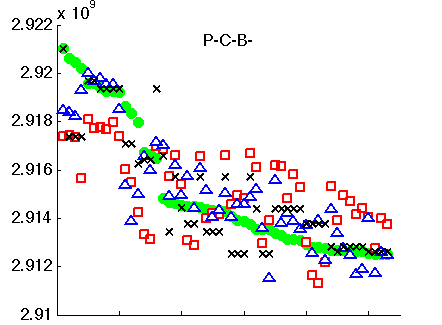
\includegraphics[scale = 0.34] {Figures/ooo_trainpredplot.png}
	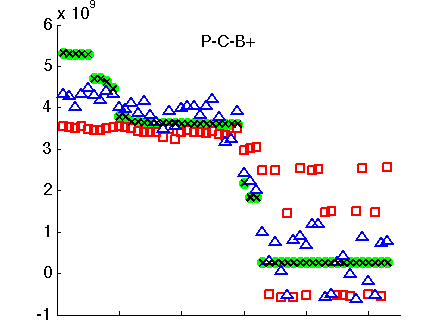
\includegraphics[scale = 0.34] {Figures/oop_trainpredplot.png}
	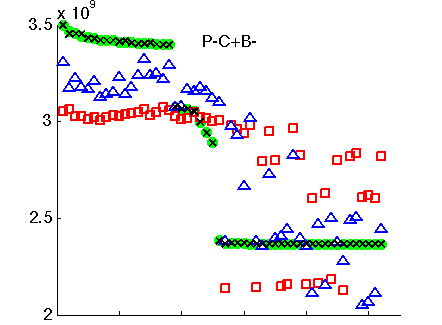
\includegraphics[scale = 0.34] {Figures/opo_trainpredplot.png}
	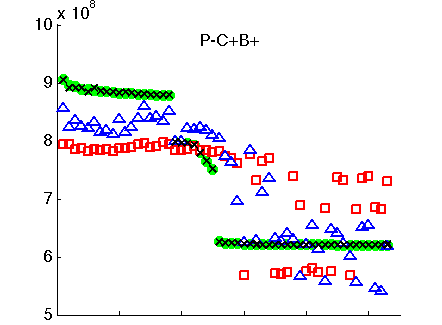
\includegraphics[scale = 0.34] {Figures/opp_trainpredplot.png}
	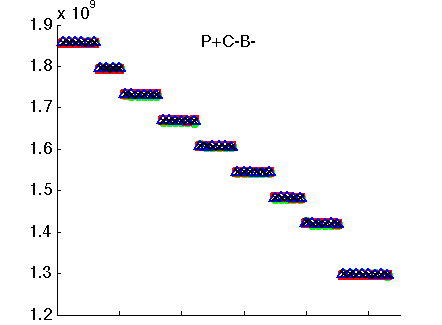
\includegraphics[scale = 0.34] {Figures/poo_trainpredplot.png}
	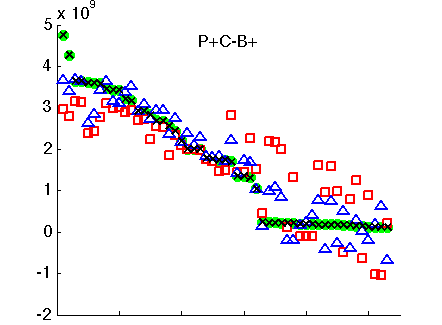
\includegraphics[scale = 0.34] {Figures/pop_trainpredplot.png}
	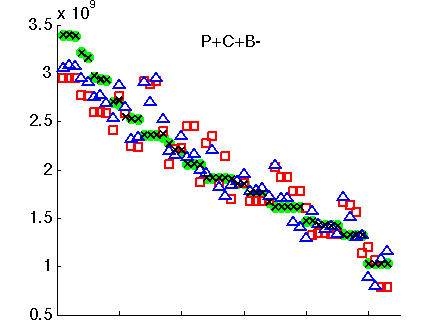
\includegraphics[scale = 0.34] {Figures/ppo_trainpredplot.png}
	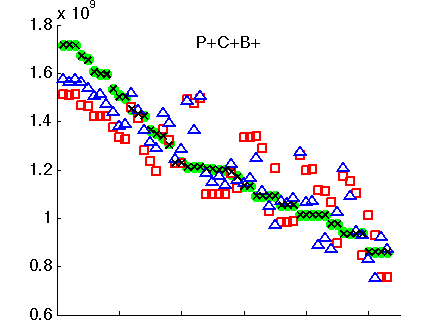
\includegraphics[scale = 0.34] {Figures/ppp_trainpredplot.png} \\
	
\includegraphics[scale = 0.5] {Figures/acc_comp_legend_horz.png}
	\caption{ \small Comparison of model accuracy for the eight microbenchmarks when predicting runtime in cycles. Each point represents a prediction for a machine configuration, and points are ordered along the x-axis based on decreasing measured run time. Y-axis plots predicted or measured runtime in cycles; note the differing ranges. In most cases, the nonlinear GPRS--based model is so accurate that it precisely captures all sample points.}
	\label{fig:acc}
\end{figure*}

%%\subsection{Partitioning Mechanism Efficacy}
%%It is worth noting that conflicts between different applications will always be destructive to performance and predictability.  The only danger to performance presented by hardware partitioning is the possibility of resource fragmentation, in which an application is allocated more of a resource than it can actually use.  However, a conservative allocation policy combined with fair sharing of excess resources can significantly mitigate this problem.

\subsubsection*{Evaluation of Model Accuracy}
In this section we examine the accuracy afforded by both the different linear regression models and the nonlinear GPRS--based regression model.  We choose a sample of 55 points from the space of 19200 possible allocations (or 0.3\%), and we train the models using this sample set.  The sample points were chosen using an Audze-Eglais DOE.

We evaluate the accuracy of the model relative to measured performance on a set of points disjoint from the sample set.  Due to the length of our simulations, we cannot exhaustively compare to all possible allocations and so limit our model error analysis to a testing set of 10 randomly selected points.  We perform this analysis for several performance metrics captured from simulation, including runtime in cycles, number of instructions committed, number of cache accesses, and number of off-chip memory accesses.

 Figure~\ref{fig:acc} plots the predictions versus measured data of a single performance metric for the sample set. While linear and nonlinear models perform equally well for some benchmarks, the nonlinear model is significantly more accurate at predicting others. The linear models struggle to capture the performance cliffs inherent to some benchmarks, especially those which move between being cache size-limited and bandwidth-limited.  In particular benchmarks which encounter a cliff and then saturate (such as the working set fitting in cache) are not faithfully modeled by the linear models.  The nonlinear model has no such difficulty.  It is also worth noting that the amount of error introduced in the linear additive and quadratic model causes them to predict negative values for some benchmarks.

\begin{table}
\small
\begin{tabular}{|l|c|c|c|}
\hline
Name & Additive & Quadratic & GPRS \\ \hline
 p--c--b-- & 0.06\% (0.04) & 0.04\% (0.04) &0.02\% (0.02) \\ \hline
 p--c--b+ &   234.07\% (287.44) & 139.21\% (167.10) &  0.23\% (0.40)   \\ \hline
 p--c+b-- &  12.67\% (5.30) &  8.26\% (5.30) &  0.02\% (0.02) \\ \hline
 p--c+b+ &  12.04\% (5.09) &  7.83\% (4.69) & 0.06\% (0.06)  \\ \hline
 p+c--b-- &  0.07\% (0.05) &  0.05\% (0.06)  &  0.05\% (0.03)  \\ \hline
 p+c--b+ &  271.05\% (377.53) & 164.23\% (226.23) & 0.51\% (1.08) \\ \hline
 p+c+b--&  13.08\% (6.91) & 8.79\% (7.32) & 0.06\% (0.07) \\ \hline
 p+c+b+&  12.07\% (4.86) &  8.05\% (5.49) & 0.08\% (0.06)  \\ \hline
   \end{tabular}
 \caption{Means (standard deviations) of percentage error in runtime cycles for each of the predictive models for each of the microbenchmarks.}
\label{table:acc-cycles}
\end{table}

\begin{table}
\small
\begin{tabular}{|l|c|c|c|}
\hline
Name & Additive & Quadratic & GPRS \\ \hline
 cluster &  4.27\% (3.66) & 6.90\% (5.67)  & 15.52\% (10.36)  \\ \hline
 gaussian&  1.83\% (0.72) & 4.16\% (2.49) & 2.33\% (3.19)  \\ \hline
 update&  4.98\% (3.04) & 7.94\% (7.12)  & 5.89\% (5.09)  \\ \hline
 pruning&  2.27\% (1.08) & 10.70\% (10.29)  & 3.07\% (2.91)  \\ \hline
 epsilon &  3.88\% (4.01) & 4.66\% (4.27)  & 2.69\% (1.09)  \\ \hline
   \end{tabular}
 \caption{Means (standard deviations) of percentage error in runtime cycles for each of the predictive models for each of the phases of the LVSRC application.}
\label{table:acc-cycles-lvsrc}
\end{table}

\begin{table}
\scriptsize
\begin{tabular}{|l|c|c|c|}
\hline
Name & Additive & Quadratic & GPRS \\ \hline
  p--c--b-- & 392.11\% (398.89) &  240.12\% (261.72) & 7.42\% (16.80)  \\ \hline
 p--c--b+ &  138133\% (290142)&  105682\% (248332) &  253.46\% (418.27)  \\ \hline
 p--c+b-- &   37225\% (65356) &  25797\% (47989) & 84.31\% (74.62)  \\ \hline
 p--c+b+ &   45276\% (82816) &  21819\% (30963) &  87.84\% (209.33)  \\ \hline
 p+c--b-- & 236.30\% (261.31) &  121.44\% (124.23) & 15.27\% (14.80)    \\ \hline
 p+c--b+ &   101696\% (169812)  &  73241\% (117426) & 25.42\% (31.95) \\ \hline
 p+c+b--&  16920\% (22871)&   12517\% (19362) & 7.47\% (8.25)  \\ \hline
 p+c+b+&   9480\% (11542) &  6647\% (9164) &  22.12\% (26.14)  \\ \hline
  \end{tabular}
 \caption{Means (standard deviations) of percentage error in offchip accesses for each of the predictive models for each of the microbenchmarks.}
\label{table:acc-offchip}
\end{table}

\begin{table}
\small
\begin{tabular}{|l|c|c|c|}
\hline
Name & Additive & Quadratic & GPRS \\ \hline
 p--c--b-- & 0.03\% (0.04) & 0.03\% (0.05) & 0.28\% (0.36) \\ \hline
 p--c--b+ & 241.91\% (262.05)  & 218.93\% (382.43) &  0.1\% (0.07) \\ \hline
 p--c+b-- & 8.49\% (5.49) & 6.17\% (6.50) & 0.41\% (1.13) \\ \hline
 p--c+b+ & 8.01\% (5.2)  & 5.79\% (6.11) & 0.07\% (0.06) \\ \hline
 p+c--b-- & 7.28\% (10.50)  & 0.05\% (0.04) & 0.27\%(0.19) \\ \hline
 p+c--b+ & 233.26\% (250.1) & 153.10\% (234.34) &  4.89\% (12.97)\\ \hline
 p+c+b-- & 20.23\% (24.18)  & 5.10\% (4.26) &  0.30\% (0.28) \\ \hline
 p+c+b+ & 13.30\% (10.23)  & 5.25\% (4.77)  & 0.05\% (0.03) \\ \hline
  \end{tabular}
 \caption{Means (standard deviations) of percentage error in cache transaction counts for each of the predictive models for each of the microbenchmarks.}
\label{table:acc-cache}
\end{table}

%\begin{table}
%\small
%\begin{tabular}{|l|c|c|c|}
%\hline
%Name & Cycles &Offchip Accesses &Cache Accesses \\ \hline
% p--c--b-- & 0.06\% (0.04) &  392.11\% (398.89) & 0.03\% (0.04) \\ \hline
% p--c--b+ &   234.07\% (287.44) & 138133\% (290142) & 241.91\% (262.05)  \\ \hline
% p--c+b-- &  12.67\% (5.30) & 37225\% (65356) & 8.49\% (5.49)  \\ \hline
% p--c+b+ &  12.04\% (5.09) &  45276\% (82816) & 8.01\% (5.2)  \\ \hline
% p+c--b-- &  0.07\% (0.05) &  236.30\% (261.31) & 7.28\% (10.50)  \\ \hline
% p+c--b+ &  271.05\% (377.53) & 101696\% (169812) & 233.26\% (250.1)  \\ \hline
% p+c+b--&  13.08\% (6.91) & 16920\% (22871) & 20.23\% (24.18)  \\ \hline
% p+c+b+&  12.07\% (4.86) &  9480\% (11542) & 13.30\% (10.23)  \\ \hline \hline
% cluster &  1 (1) & 1 (1)  & 1 (1)  \\ \hline
% gaussian&  1 (1) & 1 (1) & 1 (1)  \\ \hline
% update&  1 (1) & 1 (1)  & 1 (1)  \\ \hline
% pruning&  1 (1) & 1 (1)  & 1 (1)  \\ \hline
% epsilon &  1 (1) & 1 (1)  & 1 (1)  \\ \hline
% \end{tabular}
% \caption{Means (standard deviations) of percentage error for each of the performance measures for each of the benchmarks, as predicted by the linear response surface model.}
%\label{table:acc-lin}
%\end{table}
%
%\begin{table}
%\small
%\begin{tabular}{|l|c|c|c|}
%\hline
%Name & Cycles &Offchip Accesses &Cache Accesses \\ \hline
% p--c--b-- & 0.04\% (0.04) &  240.12\% (261.72) & 0.03\% (0.05) \\ \hline
% p--c--b+ &  139.21\% (167.10) &  105682\% (248332) & 218.93\% (382.43)  \\ \hline
% p--c+b-- &  8.26\% (5.30) &  25797\% (47989) & 6.17\% (6.50)  \\ \hline
% p--c+b+ &  7.83\% (4.69) &  21819\% (30963) & 5.79\% (6.11)  \\ \hline
% p+c--b-- &  0.05\% (0.06) &  121.44\% (124.23) & 0.05\% (0.04)  \\ \hline
% p+c--b+ &  164.23\% (226.23) &  73241\% (117426) & 153.10\% (234.34)  \\ \hline
% p+c+b--&  8.79\% (7.32) &   12517\% (19362) & 5.10\% (4.26)   \\ \hline
% p+c+b+&  8.05\% (5.49) &  6647\% (9164) & 5.25\% (4.77)  \\ \hline \hline
% cluster &  1 (1) & 1 (1) & 1 (1)  \\ \hline
% gaussian&  1 (1) & 1 (1) & 1 (1)  \\ \hline
% update&  1 (1) & 1 (1) &  1 (1)  \\ \hline
% pruning&  1 (1) & 1 (1) & 1 (1)  \\ \hline
% epsilon &  1 (1) & 1 (1) &  1 (1)  \\ \hline
% \end{tabular}
% \caption{Means (standard deviations) of percentage error for each of the performance measures for each of the benchmarks, as predicted by the quadratic response surface model.}
%\label{table:acc-quad}
%\end{table}
%
%\begin{table}
%\small
%\begin{tabular}{|l|c|c|c|}
%\hline
%Name & Cycles &Offchip Accesses &Cache Accesses \\ \hline
% p--c--b-- & 0.02\% (0.02) &   7.42\% (16.80) & 1 (1) \\ \hline
% p--c--b+ &  0.23\% (0.40) &  253.46\% (418.27) & 1 (1)  \\ \hline
% p--c+b-- &  0.02\% (0.02) &  84.31\% (74.62) & 1 (1)  \\ \hline
% p--c+b+ &  0.06\% (0.06) &  87.84\% (209.33) & 1 (1)  \\ \hline
% p+c--b-- &  0.05\% (0.03) &  15.27\% (14.80) & 1 (1)  \\ \hline
% p+c--b+ &  0.51\% (1.08) &  25.42\% (31.95) & 1 (1)  \\ \hline
% p+c+b--&  0.06\% (0.07) &  7.47\% (8.25)) & 1 (1)  \\ \hline
% p+c+b+&  0.08\% (0.06) &  22.12\% (26.14) & 1 (1)  \\ \hline \hline
% cluster &  1 (1) & 1 (1) &  1 (1)  \\ \hline
% gaussian&  1 (1) & 1 (1) & 1 (1)  \\ \hline
% update&  1 (1) & 1 (1)  & 1 (1)  \\ \hline
% pruning&  1 (1) & 1 (1) & 1 (1)  \\ \hline
% epsilon &  1 (1) & 1 (1) & 1 (1)  \\ \hline
% \end{tabular}
% \caption{Means (standard deviations) of percentage error for each of the performance measures for each of the benchmarks, as predicted by the GPRS model.}
%\label{table:acc-nonlin}
%\end{table}

Table~\ref{table:acc-cycles} reports the mean and standard deviation of percentage error of each of the models in predicting runtime cycles versus the measured performance of the test set. Table~\ref{table:acc-offchip} does the same for the off-chip accesses metric and Table~\ref{table:acc-cache} for the L2 cache transactions metric.  Points in the test set are not in the training set.

For some performance metrics the quadratic response surface models do a poor job of capturing the performance behavior of the points in the test set.  Linear additive model performance is even worse than the quadratic model, due mainly to the fact the the additive models lack interaction terms. However, the nonlinear models accurately capture the performance behavior of all metrics in most cases, with only a trouble areas, discussed below.

For all benchmarks, the number of instructions was relatively easy to predict, while the off-chip bandwidth and number of cache accesses were much more difficult.  Performance (cycles) prediction accuracy fell in between.  The benchmarks with the worst standard deviations had several extreme outliers that reduced the mean accuracy. Since the accuracy reported in the aforementioned tables is {\em percentage} error, it is subject to inflation when some absolute values being predicted are small relative to others in the set, which is the case particularly for off-chip bandwidth measurements.  Therefore, our judgement of model quality is dependent on how much we value accurate prediction of these small values.  For example, the GPRS--based model of microbenchmark \texttt{  p--c--b+}'s offchip accesses has a percentage error of 253.46\%, but this is caused by mispredictons of less than 5000 accesses (versus up to 2 million accesses incurred by the benchmark for certain resource allocations).

Our target machine runs Linux, which can add some non-determistic performance to the experiments.  A system with two-level scheduling would mostly likely see improved model accuracy.

While certain benchmarks are more challenging than others, there is no substantial difference in prediction accuracy between the synthetic benchmarks and real application. Table~\ref{table:acc-cycles-lvsrc} shows the accuracy of predictions of runtime (in cycles) per phase in terms of percentage error when measured against a test set.  The phases of the LVSRC application were actually more easily predicted than some of the microbenchmarks.  Due to the extreme length of the application (which was run to completion), the space of allocations we considered was limited to a maximum of two cores.  We reduced the size of the sample set correspondingly.  As a result, Table~\ref{table:acc-cycles-lvsrc} reflects models tuned on very small samples; with some adjustment of the genetic search parameters to prevent overfitting, all of the GPRS--based model percentage errors were reduced below 2\%.

%%For all of the applications, we can see that the models captured the performance of 90\% of the test points with less than []\% error.  This result leads us to believe that the model is an adequate enough representation of application performance to be useful in predicting performance for the remainder of the allocation options.

Clearly, the nonlinear models are extremely accurate and would make excellent input to our spatial resource allocation algorithm.  However, the GPRS--based models used here took between 0.5 and 6 hours each to build, so clearly they would have to be created offline and stored for use at runtime.  The linear models can be trained extremely rapidly, but are less accurate.  The true metric of whether or not a model is accurate ``enough'' depends on the quality of the decisions made based on it.
%We investigate decisions based on both linear and nonlinear model in Section~\ref{sec:decisions}.

\subsubsection*{Effect of Sample Size on Model Accuracy}
\label{sec:eval:acc-sample}

Figure ~\ref{fig:acc-sample} shows the impact that changing the sample set size has on model accuracy, using the example of execution time predictions for the microbenchmarks.  It is worth noting that while the accuracy of the quadratic and  nonlinear models improve rapidly with increasing sample size, the linear additive model sees no improvement on average.  This failure to improve when exposed to additional data indicates that it is the {\em form} of the model itself which is flawed (i.e. too simplistic).  Another important feature is that as sample size increases, the improvement seen by the other models slows, indicating a point of diminishing returns for increasing sample size.

This sample size analysis informs our decision about whether we can afford to use online or offline, linear or nonlinear models.  On the one hand, GPRS--based nonlinear models are much more accurate even when given smaller sample sizes.  However, they take a long time to train, and cannot be rapidly adapted to account for new data points.  On the other hand, linear models of sufficient complexity require more points to succeed, but can be rapidly trained and retrained.  A hybrid approach, in which genetic programming is used to construct the form of the response surface model offline, and then the model's coefficients are retuned based on performance data collected online, may a viable way to get the best of both worlds.

\begin{figure}
	\centering
	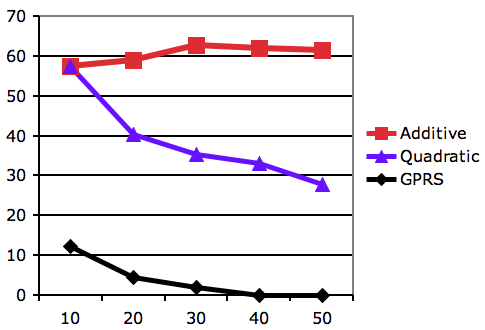
\includegraphics[scale = 0.5] {Figures/acc_sample.png}
	\caption{ \small Comparison of model accuracy for different models as training sample size is increased.  Y-axis is average percentage error in predictions of runtime averaged across all benchmarks. X-axis is increasing sample size.  Some models are more robust to reduced sample size than others.}
	\label{fig:acc-sample}
\end{figure}


\subsection{RTF Exploration and System Potential using an FPGA-based System Simulator}
~\cite{bird,tess_resource}



\subsubsection*{Experimental Setup}

We performed some of our own resource allocation experiments to
confirm that runtime hardware measurements can help improve OS
scheduling decisions.  Using an FPGA-based multiprocessor emulator RAMP Gold~\cite{rampgold09, rampgold10, fame10} and
a simple research operating system ROS~\cite{ros, tess,tess_resource}, we ran experiments with the Parsec
2.0 Benchmark Suite~\cite{parsec} and some handcrafted
microbenchmarks on a 64-core target machine. The OS uses page coloring
to allocate sections of the cache to an application, and the simulator
implements a simple form of bandwidth partitioning by limiting the
number of requests that can be sent to memory over a time
interval. Our system executes each of the applications several times,
each time varying the number of cores, and cache and bandwidth
allocations.  We collect application runtime performance data using
performance measurement hardware to create models of the performance
for that application given a particular resource allocation.  We
created a quadratic model and linear model with multivariate
regression techniques, a GPRS model, and a KCCA model using 20\% of the possible allocations.  Using
these models, our scheduler decides how best to run a mix of two
applications by trying to optimize a given objective function.  For
these results, we chose a simple proxy for total energy consumed, the
total number of cycles run (the sum of the cycles on each core) +
10$\times$ the total number of off-chip accesses, as our example
objective function.

Our experimental platform for this case study consists of five Xilinx
XUP FPGA boards. Each board is programmed to simulate one instance of
our target architecture.  Table~\ref{table:target} lists the target
machine parameters. We run six applications from the PARSEC benchmark
suite \cite{parsec}, as well as two synthetic microbenchmarks.
Table~\ref{table:benchmarks} summarizes the benchmarks. The
performance models are built based on applications running alone on a
partition of the machine but are tested against data collected from
multiprogrammed scheduling scenarios.  We simulated all possible
allocations for each benchmark running alone, and then all possible
schedules of allocations for 3 pairs of benchmarks running
simultaneously, for a combined total of 68.5 trillion target
core-cycles.  (A core-cycle is 1 clock cycle of execution on 1 core;
simulating a 64-core CMP for 1,000,000 cycles would be 64,000,000
core-cycles.)

 The Research Operating System (ROS) is a prototype operating system
 build to investigate OS design principles in the manycore era
 \cite{tess, tess_resource, tess_dac}.  We ported ROS to boot on Midas FAME, and
 modified its functionality to support our scheduling framework
 (including paging management and threading libraries).


Our spatial scheduling framework is implemented within a prototype
research operating system (ROS) that runs on the target machine
simulated by Midas FAME~\cite{ros}.


\begin{table*}[ct]
 \begin{center}
\footnotesize
\begin{tabular}{|c|l|}
\hline
 Attribute  & Setting \\ \hline \hline
 CPUs & 64 single-issue in-order cores @ \wunits{1}{GHz} \\ \hline
 L1 Instruction Cache & Private, \wunits{32}{KB}, 4-way set-associative, 128-byte lines \\ \hline
 L1 Data Cache & Private, \wunits{32}{KB}, 4-way set-associative, 128-byte lines \\ \hline
 L2 Unified Cache & Shared, \wunits{8}{MB}, 16-way set-associative, 128-byte lines, inclusive, 4 banks, \wunits{10}{ns} latency \\ \hline
 Off-Chip DRAM & \wunits{2}{GB}, 4$\times$\wunits{3.2}{GB/sec} channels,
 \wunits{70}{ns} latency \\ \hline
 \end{tabular}
\caption{Target machine parameters simulated by RAMP Gold.}
\label{table:target}
 \end{center}
\end{table*}

\begin{table*}[ct]
 \begin{center}
\footnotesize
\begin{tabular}{|l|l|l|r|l|}
\hline
 Name  & Type & Parallelism & Working Set & Bandwidth Demand\\ \hline \hline
Blackscholes & financial PDE solver & coarse data parallel & \wunits{2.0}{MB} & minimal \\ \hline
Bodytrack & vision & medium data parallel & \wunits{8.0}{MB} & grows with cores\\ \hline
Fluidanimate & animation & fine data parallel & \wunits{64.0}{MB} & grows with cores\\ \hline
Streamcluster & data mining & medium data parallel & \wunits{16.0}{MB} & high \\ \hline
Swaptions & financial simulation & coarse data parallel & \wunits{0.5}{MB} & grows with cores \\ \hline
x264 & media encoder & pipeline & \wunits{16.0}{MB} & grows with cores \\ \hline \hline
Tiny & synthetic &  one thread does all work & \wunits{1}{KB} & minimal \\ \hline
Greedy & synthetic & data parallel & \wunits{16.0}{MB} & high \\ \hline
\end{tabular}
\caption{Benchmark description. PARSEC benchmarks use \texttt{ simlarge} input set sizes, except for x264 and fluidanimate, which use \texttt{ simmedium} due to limited physical memory capacity.  PARSEC characterizations are from \cite{parsec}.}
\label{table:benchmarks}
 \end{center}
\end{table*}


\paragraph*{Partitioning Mechanisms}
Our allocation framework includes the following resources: the cores
and their private caches, the shared last-level cache, and shared
memory bandwidth.  For each resource, we provide a mechanism to
prevent applications from exceeding their allocated share. The OS
assigns cores and their associated private resources to a specific
application. For the shared last-level cache, we modify the OS
page-coloring algorithm so that applications are never given a page
from a different application's color allocation.

To partition off-chip memory bandwidth, we use Globally-Synchronized
Frames (GSF)\cite{gsf}. GSF provides strict Quality-of-Service
guarantees for minimum bandwidth and the maximum delay of a
point-to-point network---in our case the memory network---by
controlling the number of packets that each core can inject per frame.
We use a modified version of the original GSF design, which tracks
allocations per application instead of per core, does not reclaim
frames early, and does not allow applications use the excess
bandwidth.  These changes make GSF more suited to our study since we
want to strictly bound the maximum bandwidth per application.
Implementing GSF required some modifications to the target machine's
memory controller in RAMP Gold to synchronize the frames and track
application packet injections.  Due to the functional/timing split in
RAMP Gold, this modification was no more difficult than modifying a
software simulator would have been.

\paragraph{RTF Construction}

 We use a design of experiments (DoE) technique known as the Audze-Eglais
Uniform Latin Hypercube design of experiments \cite{bates-aes03} to
select the points included in the sample set.  Audze-Eglais selects
sample points which are as evenly distributed as possible through the
space of possible allocations.

To explore the relationship between model accuracy and model type
for our problem space, we evaluate linear additive models, quadratic
response surface models, and non-linear models based on Kernel Canonical Correlation Analysis (KCCA) \cite{kcca} and GPRS.

The simplest models we consider are linear additive models, which
contain one term for each variable (i.e. an allocation type) and one
coefficient associated which each term.  Linear additive models
ignore any possible interaction between the variables, an invalid
assumption in our scheduling scenario.  For this reason, we also
include more complex multivariate regression models, commonly termed
`response surface models', which include terms for variable
interaction and polynomial terms of degree 2 or more.  We also employ
Kernel Canonical Correlation Analysis (KCCA) \cite{kcca} as a
representative example of even more complex nonlinear modeling
techniques. KCCA automatically detects correlations among the
variables and outputs included in the model, and uses this analysis
to make predictions.


\paragraph{Resource Allocation Decisions}

The scheduler uses the models for each application to decide how best
to divide resources up between a mix of applications all running
concurrently.  Our initial prototype scheduler optimizes the
reassignment of spatial resource allocations without regard to the
current allocations and the resulting reallocation overhead.  Even
this simplified problem is combinatorial (and in fact is
NP-hard). The algorithm works by maximizing an objective function,
which serves to convert model outputs into a measure of overall
decision fitness.  The form of the objective function influences the
type of algorithm we can use to maximize fitness. We use Matlab's
\cite{matlab} implementation of the medium-scale active-set
algorithm, which is a sequential quadratic programming based solver
and so depends on the convexity of the function to guarantee
optimality.

Only some of our objective functions are convex, and the optimization
algorithm may choose local minima for ones which are not.  As a
result, even with perfect models the scheduler could pick non-optimal
solutions.  For this reason, it is important to experiment with
different model types, sample sizes, objective functions, and
maximization algorithms to find the right balance between system
complexity and accuracy of scheduling decisions.




\subsubsection*{Case Study Results}

\begin{figure*}[htb]
%        \center{\includegraphics[width=1.1\textwidth]
	\noindent\makebox[\textwidth]{%
        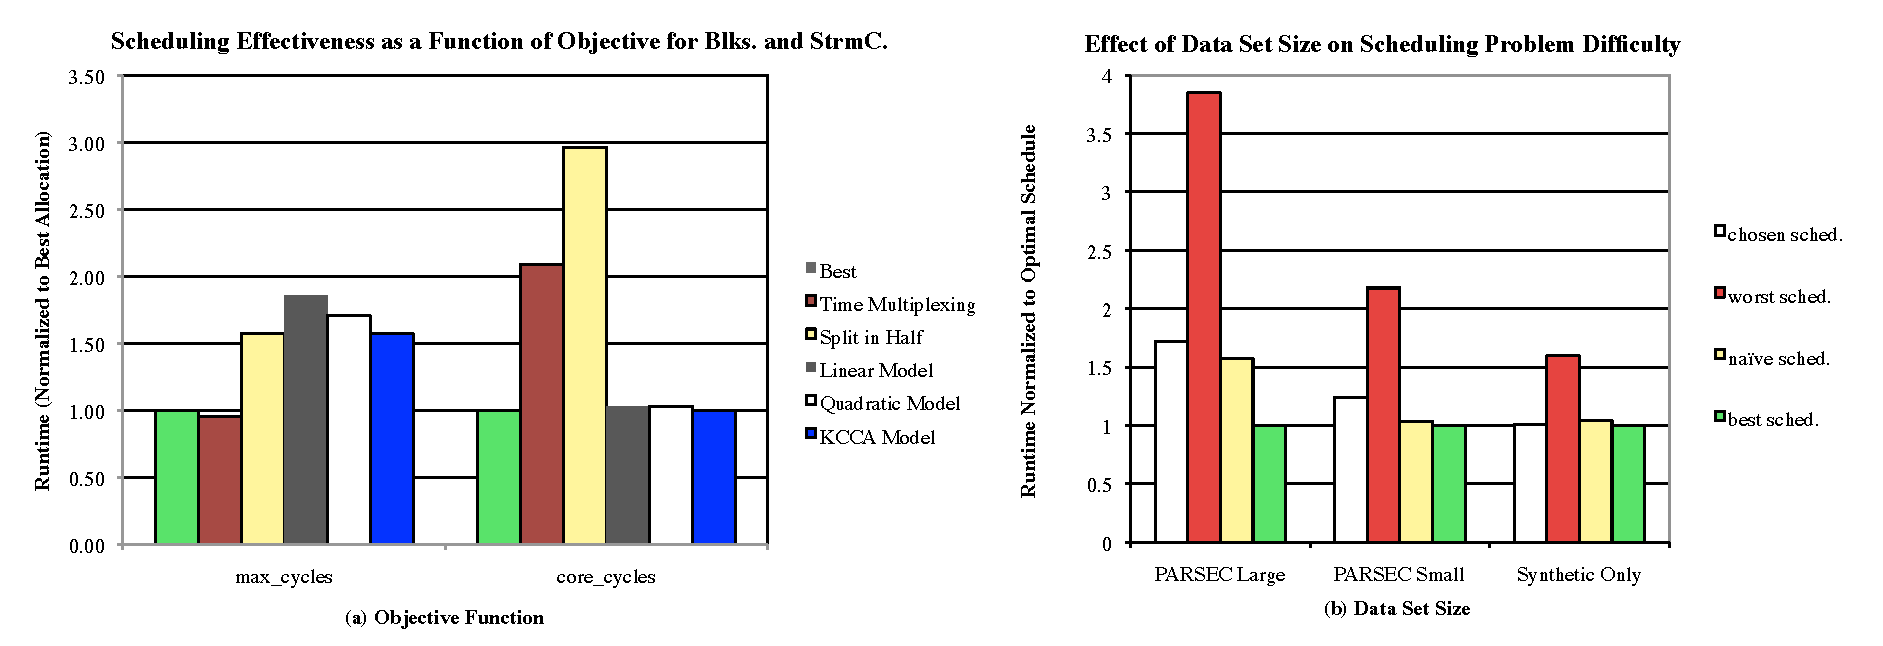
\includegraphics[width=1.0\textwidth]
        {Figures/case_study_outcome.pdf}}
        \caption{\label{fig:case_study_outcome}  (a) The performance
          of various scheduling methodologies and objective functions
          for one scheduling problem, normalized to the globally
          optimal schedule's performance.  The scheduler tries to
          minimize each objective function.  (b) The effect of
          benchmark size on the difficulty of the scheduling problem.
          The average chosen schedule performance, global worst case
          and naive scheduling case are normalized to the globally
          optimal schedule's performance for each dataset. The
          scheduling decision is Blackscholes vs. Streamcluster, the
          objective function is to minimize runtime.
 }
\end{figure*}

We found that predictive modeling has potential to successfully manage
some applications, depending on the scheduler's objective function.
For example, if the objective is to minimize energy, the approach
works quite well.  However, if the objective is to minimize the time
it takes to complete both applications, the naive baselines, such as
splitting the machine in half or time-multiplexing, often performed as
well or significantly better than model-based
allocation. Figure~\ref{fig:case_study_outcome}(a) presents an example
of these results. More importantly, our conclusions about the value of
model-based scheduling would have been different had we \emph{not}
simulated the entire execution of benchmarks, with large input sets,
for all possible allocations.

\begin{figure}[tb]
  \begin{center}
    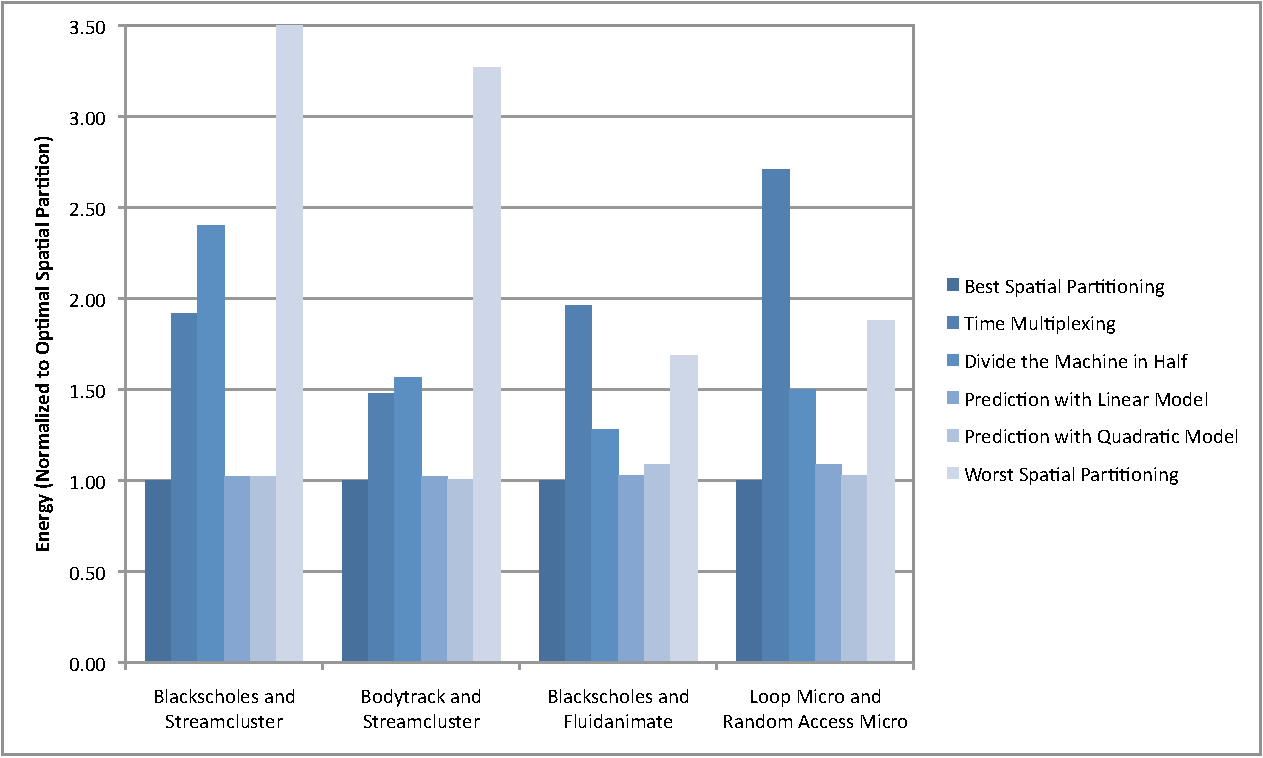
\includegraphics[width=\linewidth]{Figures/scheduling_results_energy.pdf}
  \end{center}
  \caption{Comparison of the effectiveness of different scheduling
    techniques normalized to our quadratic model-based approach.  The
    metric (sum of cycles on all cores + 10$\times$ sum of off-chip
    accesses) is a proxy for energy, so lower numbers are better.}
  \label{fig:scheduling_results}
\end{figure}




Figure~\ref{fig:scheduling_results} shows the results of our
scheduler's decisions based on the runtime performance data as
compared with several alternatives: the optimal allocation, naively
giving each application half of the machine, or time-multiplexing each
application across the entire machine.  The time-multiplexing scheme
first runs the first application to completion and then runs the
second application to completion.  More fined-grained
time-multiplexing could lead to longer runtimes due to cache
interference effects and other context swap overheads.

We do no show results for the GPRS and KCCA as we found that they were extremely non-convex and as a result often produced very poor results when paired with our optimizer. The simple linear and quadratic models perform much better with only a small set of sample points and have significantly lower overhead.

The results
show that using runtime data to perform more intelligent scheduling
can lead to a significant savings in time and energy.  Our approach
beats naively dividing the machine by 65\% and time multiplexing by
100\% on average. Furthermore, it is within a few percent of optimal
every time.  The worst-case results show that the penalty for poor
decision making can be quite large, with an energy cost 3.25$\times$
greater than our allocation on average.

As the number of cores and other shared resources grows on chip, this
will increase the number of possible allocations, thereby widening the
performance gap between good and bad schedules.  Additionally, we
expect that much more code will be tuned for parallel execution, and
exhibit a greater variety of behaviors.  As a result, there will more
likely be disjoint resource requirements among applications available
to co-schedule.  We believe hardware measurement-based scheduling will
thus prove even more effective.


\subsection{\pacora Feasibility in a Real System}
Our static framework was designed to test the effectiveness of \pacora's model-based convex optimization for allocating resources.  We used it to experiment with the accuracy of different types of models and test the quality of the resource allocation decisions. Data is collected online by running application benchmarks on a recent x86 processor running Linux-2.6.36.  The measured data is processed using Python and then fed to MATLAB~\cite{matlab} to build the RTFs.  MATLAB uses the RTFs to make resource allocation decisions.  We compare performance of the chosen resource allocations with the actual measured performance of all possible resource allocations to test quality of the resource allocation decisions. We use CVX~\cite{cvx} in MATLAB to perform the convex optimization for building RTFs and making resource allocation decisions.  We chose this static approach because it let us test many applications, 44 in total, and many resource allocations rapidly.

\subsubsection{Platform}

To collect data, we use a prototype version of Intel's Sandy Bridge x86 processor that is similar to the
commercially available client chip, but with additional hardware
support for way-based LLC partitioning.
The Sandy Bridge client chip has 4 quad-issue out-of-order
superscalar cores, each of which supports 2 hyperthreads using
simultaneous multithreading~\cite{IntelRefManual:2011}.
%Each core has private \wunits{32}{KB} instruction and data caches, as well as a
%\wunits{256}{KB} private non-inclusive L2 cache.
The LLC is a 12-way
set-associative \wunits{6}{MB} inclusive L3 cache, shared among all
cores using a ring-based interconnect.
%All three cache levels are write-back.
The cache partitioning mechanism is way-based and works by modifying the
cache-replacement algorithm.  To allocate cache ways, we assign a subset of
the 12 ways to a set of hyperthreads, thereby allowing only those hyperthreads to replace data in those ways.

%Way allocations can be completely private,
%completely shared, or overlapping.  Although all cores can hit on data stored in
%any way, a core can only replace data in its assigned
%ways.   Data is not flushed when the way allocation changes.

We use a customized BIOS that enables the cache partitioning
mechanism, and run unmodified Linux-2.6.36 for all of our experiments.
To allocate cores, we use the Linux \texttt{taskset} command to pin applications to
sets of hyperthreads. The standard Linux scheduler performs the scheduling for applications within these containers of hyperthreads. For our experiments we consider each hyperthread to be an independent core. To minimize inter-application interference, we first assign both hyperthreads available in one core before moving on to the next core. For example, a 4-core allocation from \pacora represents 4 hyperthreads on 2 cores on the machine.

\subsubsection{Performance and Energy Measurement}

To measure application performance, we use the \texttt{libpfm}
library~\cite{Eranian:OLS06,Perfmon2}, built on top of the
\texttt{perf\_events} infrastructure in Linux, to
access available performance counters~\cite{Intel:Manual2012}.

To measure on-chip energy, we use the energy counters available on
Sandy Bridge to measure the consumption of  the entire socket and also
the total combined energy of cores, their private caches, and the
LLC. We access these counters using the Running Average Power Limit
(RAPL) interfaces~\cite{Intel:Manual2012}.  %The counters measure power
%at a $1/2^{16}$ second granularity.

%In addition, we use a FitPC external multimeter to measure at the wall socket the power
%consumed by the entire system, at a
%\wunits{1}{second} granularity.
%We correlate the wall power data with the data collected from the hardware energy counters
%using time stamps.  We observed less than one second of delay in these
%measurements consistently across all experiments.  Together, these
%mechanisms allow us to collect accurate energy readings over the
%entire course of an application's execution.

\subsubsection{Description of Workloads}

Our workload contains a range of applications from three different
popular benchmark suites: SPEC CPU 2006~\cite{SPEC2006},
DaCapo~\cite{dacapo}, and PARSEC~\cite{parsec}. We selected this set of applications to represent a wide variety of possible resource behaviors in order to properly stress \pacora's RTFs. We include some additional applications to broaden the
scope of the study, and some microbenchmarks to exercise certain
system features.

The \textbf{SPEC CPU2006} benchmark suite~\cite{SPEC2006} is a
CPU-intensive, single-threaded benchmark suite, designed to stress a
system's processor, memory subsystem, and compiler.  Using the
similarity analysis performed by Phansalkar \emph{et
al.}~\cite{Phansalkar:ISCA2007}, we subset the suite, selecting 4
integer benchmarks (\texttt{ astar}, \texttt{ libquantum}, \texttt{ mcf}, \texttt{ omnetpp}) and 4
floating-point benchmarks (cactusADM, calculix, lbm, povray).  Based
on the characterization study by Jaleel~\cite{Jaleel:TR2007}, we also
pick 4 extra floating-point benchmarks that stress the LLC: \texttt{ GemsFDTD},
\texttt{ leslie3d}, \texttt{ soplex} and \texttt{ sphinx3}.  When multiple input sets are
available, we pick the single \textit{ref} input indicated by~\cite{Phansalkar:ISCA2007}.

We include the \textbf{DaCapo} Java benchmark suite as a
representative of managed-language workloads. We use the latest 2009 release, which consists of a set of open-source, real-world
applications with non-trivial memory loads, and includes both client and
server-side applications.

The \textbf{PARSEC} benchmark suite is intended to be representative
of parallel real-world applications~\cite{parsec}. PARSEC
programs use various parallelization approaches, including data- and
task-parallelization. We use native input sets and the \texttt{ pthreads} version for all benchmarks, with the exception of
\texttt{freqmine}, which is only available in OpenMP.

We add four \textbf{additional parallel applications} to help ensure
we cover the space of interest: \texttt{ Browser\_animation} is a
multithreaded kernel representing a browser layout animation; \texttt{
  G500\_csr} code is a breadth-first search algorithm; \texttt{ Paradecoder} is a parallel
speech-recognition application that takes audio waveforms of human
speech and infers the most likely word sequence intended by the
speaker; \texttt{ Stencilprobe} simulates heat transfer in a fluid
using a parallel stencil kernel over a regular
grid~\cite{Kamil:Stencilprobe}.

We also add two \textbf{microbenchmarks} that stress the memory
system and cause increased interference between applications: \texttt{ stream\_uncached} is a memory and on-chip bandwidth hog
that continuously brings data from memory without caching it, while
\texttt{ ccbench} explores arrays of different sizes to determine the
structure of the cache hierarchy.

Using a performance characterization of the applications, we select a subset of the benchmarks that are representative of different possible responses to resource allocations in order to reduce our study to a feasible size.  Similar to \cite{Phansalkar:ISCA2007}, we use machine learning to select representative benchmarks.  We use a
hierarchical clustering algorithm~\cite{Phansalkar:ISCA2007} provided by the Python library \texttt{scipy-cluster} with the \textit{single-linkage} method.  The feature vector contains parameters to represent core scaling, cache scaling, prefetcher sensitivity and bandwidth sensitivity.  The clustering algorithm uses Euclidean distance between vectors to determine clusters.

The clustering results in 6 clusters representing the following (applications at the cluster center are listed in parenthesis):
 \begin{itemize}\itemsep0pt \parskip0pt \parsep5pt
\item no scalability, high cache utility, (\texttt{ 429.mcf})
\item no scalability, low cache utility, (\texttt{ 459.gems\-FDTD})
\item high scalability, low cache utility, (\texttt{ ferret})
\item limited scalability, high cache utility, (\texttt{ fop})
\item limited scalability, low cache utility, (\texttt{ dedup})
\item limited scalability, low bandwidth sensitivity, (\texttt{ batik})
\end{itemize}

%First, we create a feature vector for each application using the values in the previous subsection:
%1) execution time as we increase the number of threads; 2) execution time as we increase the LLC size; 3) prefetcher sensitivity; and 4) bandwidth sensitivity. All metrics are normalized to the interval $[0,1]$. In total we use vectors with 19 features ($7+10+1+1$).

%The clustering algorithm finds the smallest Euclidean distance of a pair of feature vectors and forms a cluster containing that pair. It continues selecting the next smallest distance between a pair and forms another cluster. Linkage criteria can be used to adjust cluster formation. The single-linkage we selected uses the minimum distance between a pair of objects in different clusters to determine the distance between them.

\subsubsection{RTF Experiments}
\begin{figure*}[!t]
	\begin{center}	
		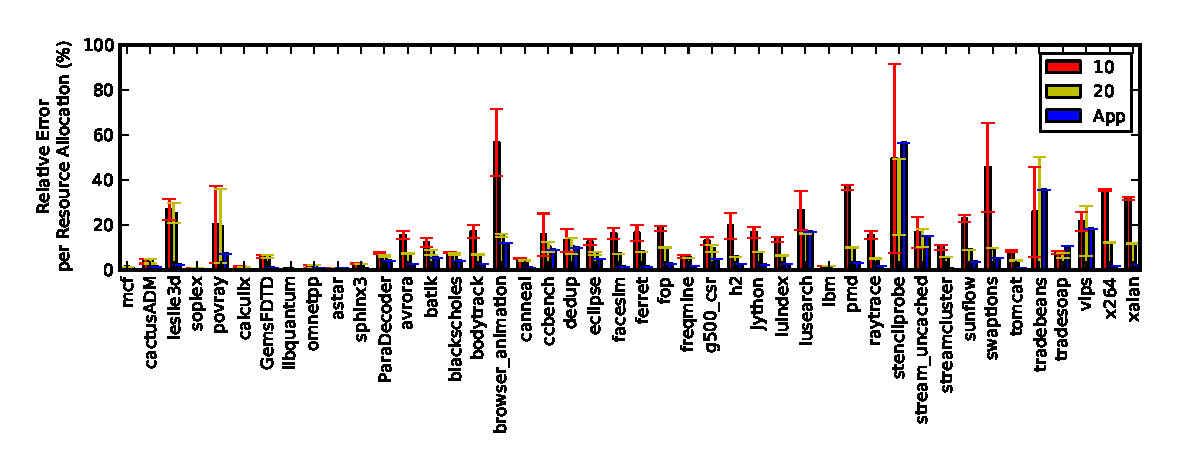
\includegraphics[bb=0 0 576 216,width=\textwidth]{Figures/model_accuracy.pdf}
		\caption{1-norm of relative error from RTF predicted response time compared to actual response time.  The actual response time is the median over 3 trials. 10 and 20 represent RTFs built with 10 and 20 training points respectively.  App represents the variability (average standard deviation) in performance of the application between the 3 trials.}
		\label{model_accuracy}
	\end{center}
\end{figure*}
To test the effectiveness of our RTFs in capturing real application behavior, we measure each of our 44 benchmarks running alone on the machine for all possible resource allocations of cache ways and cores.  Cores can be allocated from 1--8 and cache ways from 1--12 resulting in 96 possible allocations for each application.   We use a genetic algorithm design of experiments~\cite{bates-aes03} to select 10 and 20 of the collected allocations to build the RTFs.  We also experimented with building RTFs with more data points but found that they provided little improvement over 20~\cite{pacora_tr}.  We then use the model to predict the performance of every resource allocation and compare it with the actual measured performance (median value of 3 trials) of that resource allocation.  We built 3 different models from 3 trials and tested each of them against median measured value.

Figure~\ref{model_accuracy} shows the 1-norm of the relative error of the predicted response times per resource allocation for an RTF built with 10 training points and one built with 20.  The average error per point is 16\% for an RTF built with 10 training points and 9\% for an RTF built with 20 training points.  We also calculated the percentage variability (average standard deviation) for each resource allocation in the application between the 3 trials (shown as ``App'' in Figure~\ref{model_accuracy}).  The average variability is 9\%, so we can see that \pacora's RTFs are not much more inaccurate than the natural variation in response time in the application.  It is not for possible an RTF to be more accurate than the application variability, and we can also see that applications with higher variability result in RTFs with larger relative errors, (\emph{e.g.,} \texttt{stencilprobe}, \texttt{ tradebeans}).  Section~\ref{discuss} discusses application variability in more detail.

\subsubsection{Resource Allocation Experiments}
\begin{figure}[!t]
	\begin{center}	
		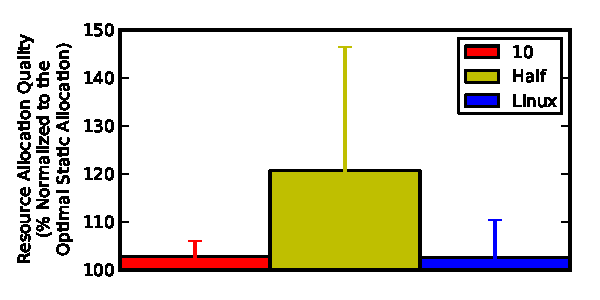
\includegraphics[bb=0 0 288 144,width=\columnwidth]{Figures/decision_quality.pdf}
		\caption{Resource allocation decisions for each pair of the cluster representative applications compared equally dividing the machine and a shared resources Linux baseline. Quality is measured is allocation performance divided by performance of the best possible allocation.}
		\label{decision_quality}
	\end{center}
\end{figure}


Using the RTFs built for the applications, we let \pacora make static resource allocations for all possible pairs of the cluster representative applications.  We then run an exhaustive study of all possible resource allocations for each pair on our Sandy Bridge-Linux platform, measure the performance, and compare it with the best performing, \emph{i.e.,} optimal, resource allocation.  We also compare this result to equally dividing the resources between the two applications and to sharing all of the resources using the standard Linux scheduler.

%how \pacora's decisions compared with the optimal allocation, equally dividing the machine, and the Linux baseline for each pair of the cluster representative applications.
Figure~\ref{decision_quality} shows these results for our 10 point RTFs. As we might expect, simple naive heuristics do not perform well, and dividing the machine in half is around 20\% slower than either \pacora or standard Linux.
 \pacora's resource allocations are 2\% from the optimal static allocation on average.  Using shared resources with the standard Linux scheduler performs similarly but with a higher standard deviation.  The shared resources comparison is interesting: while most of the time sharing resources can result in higher utilization, as the applications can dynamically take advantage of available resources, in some cases the interference between applications was so harmful to performance that on average optimal static partitioning performs slightly better.  As a result \pacora is able to provide performance comparable to Linux scheduling on shared resources with more predictable performance on average (lower worst cases).  Additionally, as the shown in the next Section, \pacora's resource allocation decisions do not need to be static, but can be made dynamically to adjust to the changing needs of the applications.
%These results indicate the \pacora is able to get a near optimal resource allocation and match the performance of the traditional Linux scheduler with more predictability.

\subsubsection{Effect of Model Accuracy on Decision Quality}

\begin{figure}[!t]
	\begin{center}	
%		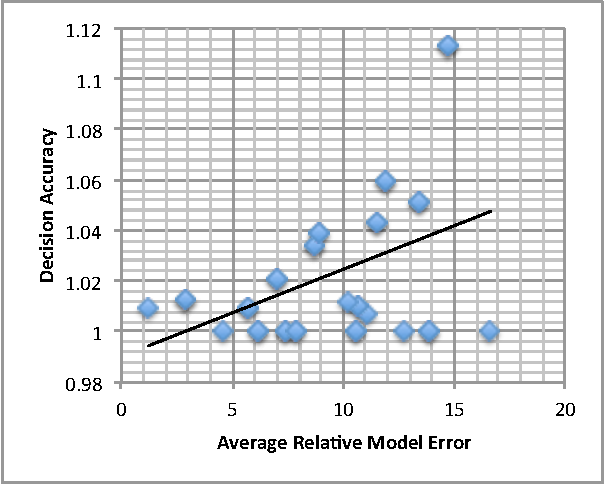
\includegraphics[width=0.9\textwidth]{cluster_decision_accuracy.pdf}
		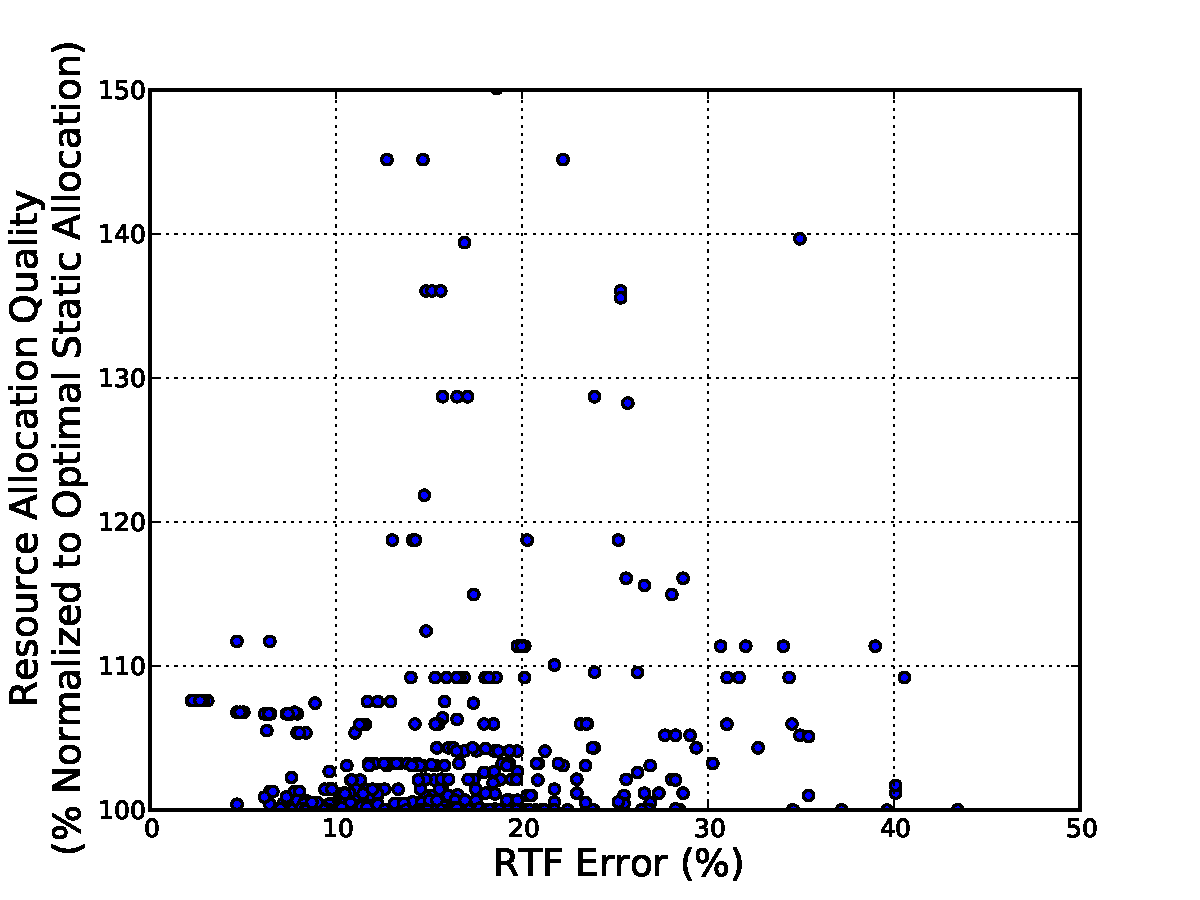
\includegraphics[bb=0 0 576 432,width=\columnwidth]{Figures/accuracy_quality.pdf}
		\caption{Effect of Model Accuracy on Decision Quality. The x axis represents the combined relative error of all RTFs used in the decision.}
		\label{accuracy_quality}
	\end{center}
\end{figure}


There are two main sources of challenges for \pacora's design: performance non-convexity and performance variability. 
The main concern with performance non-convexity and variability is their effects on the accuracy of the response time functions.  However, an important result we have found while evaluating \pacora is that model accuracy has less impact on the quality of resource allocation decisions than we anticipated.  When experimenting with possible models for the RTFs, we found that while some models were always a little too inaccurate and did degrade the performance of the resource allocation decisions, once a model crossed a certain threshold of accuracy then better models provided insignificant improvement in resource allocation decisions. Figure~\ref{accuracy_quality} shows the effect of model accuracy on the quality of the resource allocation decisions made using the RTF model in Equation~\ref{rtf_eq}.  Although there is a slight correlation between model accuracy and decision quality, many decisions with inaccurate models still result in near optimal allocations.  This effect enables \pacora's model-based design to be feasible in a noisy system with real applications.
